% DPF 09 talk on strangeness in nucleon

\documentclass[10pt]{beamer}
\usefonttheme{professionalfonts} % using non standard fonts for beamer
\usefonttheme{serif} % default family is serif
\usepackage{amsmath}
\usepackage{ulem}
\usepackage{array}
\usepackage{mathtools}
%\documentclass[12pt]{beamerthemeSam.sty}
\usepackage{epsf}
%\usepackage{pstricks}
%\usepackage[orientation=portrait,size=A4]{beamerposter}
\geometry{paperwidth=160mm,paperheight=120mm}
%DT favorite definitions
\def\LL{\left\langle}	% left angle bracket
\def\RR{\right\rangle}	% right angle bracket
\def\LP{\left(}		% left parenthesis
\def\RP{\right)}	% right parenthesis
\def\LB{\left\{}	% left curly bracket
\def\RB{\right\}}	% right curly bracket
\def\PAR#1#2{ {{\partial #1}\over{\partial #2}} }
\def\PARTWO#1#2{ {{\partial^2 #1}\over{\partial #2}^2} }
\def\PARTWOMIX#1#2#3{ {{\partial^2 #1}\over{\partial #2 \partial #3}} }

\def\rightpartial{{\overrightarrow\partial}}
\def\leftpartial{{\overleftarrow\partial}}
\def\diffpartial{\buildrel\leftrightarrow\over\partial}

\def\BI{\begin{itemize}}
\def\EI{\end{itemize}}
\def\BE{\begin{displaymath}}
\def\EE{\end{displaymath}}
\def\BEA{\begin{eqnarray*}}
\def\EEA{\end{eqnarray*}}
\def\BNEA{\begin{eqnarray}}
\def\ENEA{\end{eqnarray}}
\def\EL{\nonumber\\}
\def\BS{\bigskip}
\def\BC{\begin{center}}
\def\EC{\end{center}}
\def\BCC{\begin{columns}}
\def\ECC{\end{columns}}
\def\HC{\column{0.5\textwidth}}

\newcommand{\etal}{{\it et al.}}
\newcommand{\gbeta}{6/g^2}
\newcommand{\la}[1]{\label{#1}}
\newcommand{\ie}{{\em i.e.\ }}
\newcommand{\eg}{{\em e.\,g.\ }}
\newcommand{\cf}{cf.\ }
\newcommand{\etc}{etc.\ }
\newcommand{\atantwo}{{\rm atan2}}
\newcommand{\Tr}{{\rm Tr}}
\newcommand{\dt}{\Delta t}
\newcommand{\op}{{\cal O}}
\newcommand{\msbar}{{\overline{\rm MS}}}
\def\chpt{\raise0.4ex\hbox{$\chi$}PT}
\def\schpt{S\raise0.4ex\hbox{$\chi$}PT}
\def\MeV{{\rm Me\!V}}
\def\GeV{{\rm Ge\!V}}

%AB: my color definitions
%\definecolor{mygarnet}{rgb}{0.445,0.184,0.215}
%\definecolor{mygold}{rgb}{0.848,0.848,0.098}
%\definecolor{myg2g}{rgb}{0.647,0.316,0.157}
\definecolor{abtitlecolor}{rgb}{0.0,0.255,0.494}
\definecolor{absecondarycolor}{rgb}{0.0,0.416,0.804}
\definecolor{abprimarycolor}{rgb}{1.0,0.686,0.0}
\definecolor{Red}           {cmyk}{0,1,1,0}
\definecolor{Grey}           {cmyk}{.7,.7,.7,0}
\definecolor{Lg}           {cmyk}{.4,.4,.4,0}
\definecolor{Blue}          {cmyk}{1,1,0,0}
\definecolor{Green}         {cmyk}{1,0,1,0}
\definecolor{Brown}         {cmyk}{0,0.81,1,0.60}
\definecolor{Black}         {cmyk}{0,0,0,1}
\definecolor{A}{rgb}{0.8,0.0,0.0}
\definecolor{B}{rgb}{0.0,0.6,0.0}
\definecolor{C}{rgb}{0.6,0.6,0.0}
\definecolor{D}{rgb}{0.0,0.0,0.5}
\definecolor{E}{rgb}{0.4,0.4,0.4}


\usetheme{Madrid}


%AB: redefinition of beamer colors
%\setbeamercolor{palette tertiary}{fg=white,bg=mygarnet}
%\setbeamercolor{palette secondary}{fg=white,bg=myg2g}
%\setbeamercolor{palette primary}{fg=black,bg=mygold}
\setbeamercolor{title}{fg=abtitlecolor}
\setbeamercolor{frametitle}{fg=abtitlecolor}
\setbeamercolor{palette tertiary}{fg=white,bg=abtitlecolor}
\setbeamercolor{palette secondary}{fg=white,bg=absecondarycolor}
\setbeamercolor{palette primary}{fg=black,bg=abprimarycolor}
\setbeamercolor{structure}{fg=abtitlecolor}

\setbeamerfont{section in toc}{series=\bfseries}

%AB: remove navigation icons
\beamertemplatenavigationsymbolsempty
\title{
  \textbf {Moment of inertia}\\
%\centerline{}
%\centering
%\vspace{-0.0in}
%\includegraphics[width=0.3\textwidth]{propvalues_0093.pdf}
%\vspace{-0.3in}\\
%\label{intrograph}
}

\author[W. Freeman] {Physics 211\\Syracuse University, Physics 211 Spring 2022\\Walter Freeman}

\date{\today}

\begin{document}

\frame{\titlepage}

\frame{\frametitle{\textbf{Announcements}}
\large
\BI
\item Homework 8 will be posted later today
\item It will be due next Wednesday
\item You will have recitation tomorrow as usual
\EI
}

\frame{\frametitle{\textbf{Exam 3}}
	\large
    We are still grading Exam 3; we won't have it ready for you by Friday.
    
    \BS
    
    However, it looks like students' performance on this exam was somewhat lower than on the previous two exams, despite this material being simpler and with fewer nuances than the material on Exams 1 and 2.
    
    \BS\pause
    
    (We tried to make this exam pretty straightforward.)
    
    \BS\pause
    
    Why might this be? This is a genuine question.
    
    \pause
    
    \BS\BS\BS
    
    How many of you also had a calculus exam on the same day? 
}


\frame{\frametitle{\textbf{Exam 3}}
	\large
	
	We are going to give you another chance to demonstrate your knowledge of this material, since it is some of the most critical from this course for Physics 2 and for engineering.
	
	\BS\pause
	
	We are also going to make sure that nobody fails our course because of a low performance on this exam.
	
	\BS\pause
	
	To be clear:
		
	\begin{enumerate}
		\item Our standards haven't changed: we expect you to understand work, energy, power, and the conservation of momentum\pause
		\item We are going to make additional space and time for you to learn this material\pause
		\item ... and we are going to give you another chance to demonstrate your knowledge of it.
	\end{enumerate}

\BS

In short:

\BI
\item Everyone will have an opportunity to redeem low grades on this exam, even beyond what we're already doing
\item ... but you'll need to do some work toward that end.
\EI
}


\frame{\frametitle{\textbf{Exam 3: learning the material}}
	\large
	
	Part of Homework 8 will be to do Exam 3 again, as homework. {\it (You don't need to do this if you earned 80\% or higher.)}
	
	\BS
	
	This will let you earn a fraction of credit back -- the lower your original score, the more credit you can earn back. {\color{Red}\textit{(Because of the limitations on TA's time, they will be grading this somewhat quickly and not looking in detail for partial credit: we expect you to understand things fully the second time around!)}}
	
	\BS
	
	
	
	The rest of HW8 will be shorter to allow you to do that.
	
	\BS
	
	I will hold extra help hours Monday from 2:30-5pm in the Physics Clinic to help people learn this material.
}

\frame{\frametitle{\textbf{Final exam: earning credit back}}
	\large
	
	I mentioned earlier that everyone will have a second opportunity to demonstrate mastery of material that they didn't have the first time around.
	
	\BS
	
	Here's how this will work:
	
	\BS
	
	\BI
	\item The final exam will have material from throughout the semester
	
	\BS
	
	\item If you do better on the material from Unit 1, 2, or 3 on the final exam than you did on Exam 1, 2, or 3...
	
	\BS
	
	\item ... in addition to that helping you on the final exam, you will earn part of the difference back on your earlier exam. \pause
	
	\BS
	
	\item This will be structured to ensure that anyone with a passing understanding of the material at the end of the semester passes.
	\EI
}

\frame{\frametitle{\textbf{``I'm worried about my grade!'' and other FAQs}}
	

	The median grade for Exams 1 and 2 was consistent with the class median being a B+ or even A-, given the lenient grading policy.
	
	\BS\BS
	
	The median grade for Exam 3 will be lower, but most students will get a B or better in the course.
	
	
	\BS\BS\pause\color{Red}
	
\textbf{	Q: Am I going to pass this class? }\\
	A1: If you have been going to recitation and doing your homework, almost certainly. \\
	\begin{itemize}\color{Red}
		\item Remember 50\% is passing, and homework/recitation attendance is free credit
		\item If your exam grades are very low, you should identify the core skills you need to develop and work on them before the final
	\end{itemize}
	A2: If you have been earning low scores on the exams {\it and} not doing your homework/coming to recitation, maybe not
	
	\BS\BS\pause
	\color{Green}
\textbf{	Q: Can you calculate my grade for me?} \\
	A1: Yes, but you can calculate it better than I can.\\
	A2: Because of the way the final works, no matter how you have done thus far, you can earn a high grade by learning the material now
	
	\BS\BS\pause
	\color{Blue}
\textbf{	Q: I missed an exam for [good reason X], what do I do?} \\
	A1: We will arrange for you to take an abbreviated makeup exam either on the day of the final or at another time during finals week.
	
}


\frame{\frametitle{\textbf{Missed exams}}
	\large
	
	I am completely saturated with email about missed exams. I will answer it as quickly as I can, but I have too much mail right now.
}
	



\frame{\frametitle{\textbf{A final note:}}
\BC
\Large

No matter what grades you earn, we support you and will do whatever we can to --

\BS\BS


\BI
\item Ensure you are supported, welcomed, and treated with dignity\pause
\item Advocate for you at the university however we can\pause
\item Help you learn physics
\EI

\BS

No matter what, you are welcomed and valued in our class and we'll do our damndest to help you succeed; we are on your side.

\BS\BS\pause

\large

I often have students disclose mental health problems, personal issues, issues with the university administration, and worse to me.
\BS

I don't go look up their grades before doing whatever I can for them. 

\EC

}

\frame{\frametitle{\textbf{Taking stock: what have we learned?}}
	
\Large

\textbf{Unit 1:} Kinematics -- how do we describe motion, and what is acceleration?

\BS\BS\pause

\textbf{Unit 2:} Dynamics and $\vec F = m \vec a$ -- how do forces make things accelerate?

\BS\BS\pause

\textbf{Unit 3:} Conserved quantities -- energy and momentum

\BS\BS\pause

\textbf{Unit 4:} Rotation

\BS\BS\BS\pause

It turns out that rotational dynamics is mostly a mirror of what you have learned already!

}




	
	\frame{
		\begin{center}
			\begin{tabular}{l | l}
				
				\multicolumn{1}{c|}{\Large Translational Idea} & \multicolumn{1}{c}{\Large What it means} \\
				\\
				\hline
				\hline
				& \\
				Position $\vec s$ & Where is the thing? \\
				Velocity $\vec v$ & How is it moving? \\
				Acceleration $\vec a$ & How is its motion changing? \\
				& \\
				\hline
				\hline
				& \\
				Kinematics: $\vec s(t)=\frac{1}{2}\vec at^2 + \vec v_0 t + \vec s_0$ & How does accel relate to position and velocity?\\
				& \\
				\hline
				\hline
				
				& \\
				Force $\vec F$ & What pushes on the thing? \\
				Mass $m$ & How hard is the thing to move? \\
				Newton's second law $\vec F = m \vec a$ & How do forces make things move? \\
				& \\
				
				\hline
				\hline
				
				& \\
				Kinetic energy $KE=\frac{1}{2}mv^2$ & Energy associated with speed \\
				Work $W = \vec F \cdot \Delta \vec s$ & How do forces change objects' speed? \\
				Power $P = \vec F \cdot \vec v$ & At what rate do forces change objects' energy?\\
				& \\
				
				\hline
				\hline
				
				& \\
				Momentum $\vec p = m \vec v$ & The ``persistence'' of an object's motion\\
				& \\
				
				\hline
			\end{tabular}
		\end{center}
	}
	

	


\frame{
\begin{center}
\begin{tabular}{l | l}

 \multicolumn{1}{c|}{\Large Translation} & \multicolumn{1}{c}{\Large Rotation} \\
 \\
\hline
\hline
 & \\
Position $\vec s$ & Angle $\theta$ \\
Velocity $\vec v$ & Angular velocity $\omega$ \\
Acceleration $\vec a$ & Angular acceleration $\alpha$ \\
 & \\
\hline
\hline
 & \\
Kinematics: $\vec s(t)=\frac{1}{2}\vec at^2 + \vec v_0 t + \vec s_0$ & $\theta(t) = \frac{1}{2}\alpha t^2 + \omega_0 t + \theta_0$ \\
 & \\
\hline
\hline

 & \\
Force $\vec F$ & Torque $\tau$ \\
Mass $m$ & Rotational inertia $I$ \\
Newton's second law $\vec F = m \vec a$ & Newton's second law for rotation $\tau = I \alpha$ \\
 & \\

\hline
\hline

 & \\
Kinetic energy $KE=\frac{1}{2}mv^2$ & Kinetic energy $KE=\frac{1}{2}I\omega^2$ \\
Work $W = \vec F \cdot \Delta \vec s$ & Work $W = \tau \Delta \theta$ \\
Power $P = \vec F \cdot \vec v$ & Power $P = \tau \omega$ \\
 & \\

\hline
\hline

 & \\
Momentum $\vec p = m \vec v$ & Angular momentum $L = I\omega$\\
 & \\

\hline
\end{tabular}
\end{center}
}

\frame{
	\begin{center}
		\begin{tabular}{l | l}
			
			\multicolumn{1}{c|}{\Large Translation} & \multicolumn{1}{c}{\Large Rotation} \\
			\\
			\hline
			\hline
			& \\
			\color{Grey} Position $\vec s$ &\color{Grey}  Angle $\theta$ \\
		\color{Red}		Velocity $\vec v$ & \color{Red} Angular velocity $\omega$ \\
		\color{Grey} 	Acceleration $\vec a$ & \color{Grey} Angular acceleration $\alpha$ \\
			& \\
			\hline
			\hline
			& \\
		\color{Grey} 	Kinematics: $\vec s(t)=\frac{1}{2}\vec at^2 + \vec v_0 t + \vec s_0$ & \color{Grey} $\theta(t) = \frac{1}{2}\alpha t^2 + \omega_0 t + \theta_0$ \\
			& \\
			\hline
			\hline
			
			& \\
			\color{Grey} Force $\vec F$ & \color{Grey} Torque $\tau$ \\
		\color{Red}	Mass $m$ & \color{Red} Rotational inertia $I$ \\
			\color{Grey} Newton's second law $\vec F = m \vec a$ & \color{Grey} Newton's second law for rotation $\tau = I \alpha$ \\
			& \\
			
			\hline
			\hline
			
			& \\
		\color{Red}		Kinetic energy $KE=\frac{1}{2}mv^2$ & 	\color{Red}	Kinetic energy $KE=\frac{1}{2}I\omega^2$ \\
		\color{Grey} 	Work $W = \vec F \cdot \Delta \vec s$ &\color{Grey}  Work $W = \tau \Delta \theta$ \\
		\color{Grey} 	Power $P = \vec F \cdot \vec v$ &\color{Grey}  Power $P = \tau \omega$ \\
			& \\
			
			\hline
			\hline
			
			& \\
		\color{Grey} 	Momentum $\vec p = m \vec v$ & \color{Grey} Angular momentum $L = I\omega$\\
			& \\
			
			\hline
		\end{tabular}
	\end{center}
}




%\frame{\frametitle{\textbf Last time}
%
%\Large
%
%Calculating torque:
%
%$$\tau = F_\perp r = F r_\perp = Fr \sin \theta$$
%
%\BI
%\item Draw an extended force diagram
%\item Label all forces -- both where they act and what they are
%\item Write an expression for the torque applied by each
%\item Counterclockwise torques are positive; clockwise torques are negative.
%\EI
%
%If $\alpha=0$ (``static equilibrium'', ``dynamic equilibrium''):
%
%\BI
%\item This means that the net torque (about {\it any} pivot) is zero
%\item Choose a pivot on top of a force whose value you {\color{Red} don't know}
%and {\color{Red}don't care} about 
%\item \color{Red}Write down $\sum \tau = 0$ and solve
%\EI
%}
%
%\frame{
%
%\Large
%\BC
%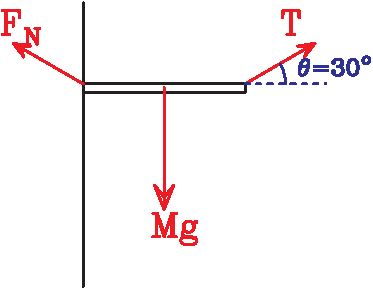
\includegraphics[width=0.5\textwidth]{beam-crop.pdf}
%
%How does the tension $T$ compare to the weight of the beam?
%
%\EC
%
%\BS
%\Huge
%\BCC
%\HC
%\color{A}A: $T \leq mg/2$ \\
%\color{B}B: $mg/2 < T < mg$ \\
%\HC
%\color{C}C: $T = mg$ \\
%\color{D}D: $mg < T < 2mg$ \\
%\ECC
%\BC
%\color{E}E: $T >=` 2mg$ \\
%\EC
%}
%
%\frame{\frametitle{\textbf{Beyond equilibrium}}
%
%
%
%\begin{center}
%\begin{tabular}{l | l}
%
% \multicolumn{1}{c|}{\Large Translation} & \multicolumn{1}{c}{\Large Rotation} \\
% \\
%\hline
%\hline
% & \\
%Position $\vec s$ & Angle $\theta$ \\
%Velocity $\vec v$ & Angular velocity $\omega$ \\
%Acceleration $\vec a$ & Angular acceleration $\alpha$ \\
% & \\
%\hline
%\hline
% & \\
%Kinematics: $\vec s(t)\frac{1}{2}\vec at^2 + \vec v_0 t + \vec s_0$ & $\theta(t) = \frac{1}{2}\alpha t^2 + \omega_0 t + \theta_0$ \\
% & \\
%\hline
%\hline
%
% & \\
%Force $\vec F$ & Torque $\tau$ \\
%Mass $m$ & Rotational inertia $I$ \\
%Newton's second law $\vec F = m \vec a$ &{\color{Red} Newton's second law for rotation $\tau = I \alpha$} \\
% & \\
%
%\hline
%\hline
%
% & \\
%Kinetic energy $KE=\frac{1}{2}mv^2$ & {\color{Red}Kinetic energy $KE=\frac{1}{2}I\omega^2$} \\
%Work $W = \vec F \cdot \Delta \vec s$ & Work $W = \tau \Delta \theta$ \\
%Power $P = \vec F \cdot \vec v$ & Power $P = \tau \omega$ \\
% & \\
%
%\hline
%\hline
%
% & \\
%Momentum $\vec p = m \vec v$ & {\color{Red}Angular momentum $L = I\omega$}\\
% & \\
%
%\hline
%\end{tabular}
%\end{center}
%}

\frame{\frametitle{\textbf{Moment of inertia}}

  \centerline{\Large The analogue of mass is called ``moment of inertia'' (letter $I$)}

  \BI
  \large
\item{More massive things are harder to turn, but that's only part of it}
\item{The mass {\it distribution} matters, too}
\item{The further the mass is from the center, the harder it will be to turn}
\item{The moment of inertia depends on the {\it average squared distance from the center}}
  \EI

  \bigskip\pause

  \centerline{\Large $I=MR^2$}

\bigskip
\bigskip
\bigskip

  \centerline{\large (if all the mass is the same distance from the center)}
  \centerline{\large (our demo rods; hoops; rings; bike wheels)}
}

\frame{\frametitle{\textbf{Moment of inertia: why?}}

\large

To see why $I=M\LL r^2\RR$, let's consider the kinetic energy of a spinning object.

\BS

The kinetic energy of a single ``point mass'' moving in a circle is 
$\frac{1}{2}mv^2 = \frac{1}{2}mr^2\omega^2$, where $r$ is its distance from the 
center.

\BS\pause

Since $KE_{\rm rot}=\frac{1}{2}I\omega^2$, this means $I=mr^2$ for a single point.

\BS\pause

For an extended object, we simply add up the energy of all the moving particles:

$$ I = \int r^2 dm = M \LL r^2 \RR$$

i.e. {\color{Red} the moment of inertia is just the total mass times the 
average squared distance from the axis.}

}

\frame{\frametitle{\textbf{Moment of inertia, other things}}
  \centerline{\Large What about the moment of inertia of other objects?}
  \centerline{\large Requires calculus in general; here are some common ones}
  \centerline{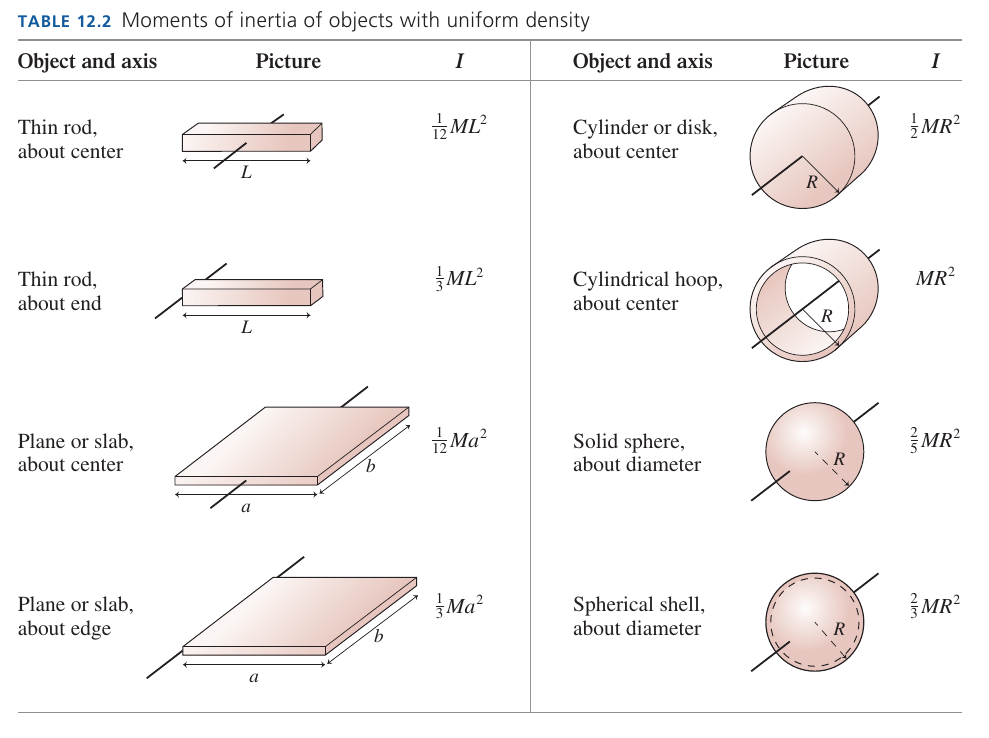
\includegraphics[width=0.7\textwidth]{moment-table.png}}

\BS
\pause
\centerline{In general: $I=\lambda MR^2$}
\centerline{We will always give you $I$ if it's not 1 (i.e. not a ring etc.)}
}
%
%\frame{\frametitle{\textbf{Newton's second law for rotation}}
%
%\Huge
%
%$$\tau = I \alpha$$
%
%\Large
%
%\BC
%
%``Newton's second law for rotation'':
%
%\BS
%
%\large
%Torques give things angular acceleration, just like forces make things accelerate.
%\EC
%}
%
%\frame{
%
%\Large
%
%Which will make the hanging object fall faster?
%
%\BS
%
%\color{A}A: Increasing the diameter of the spool the string is wound around \\
%\color{B}B: Decreasing the diameter of the spool the string is wound around \\
%\color{C}C: Moving the spinning masses inward \\
%\color{D}D: Moving the spinning masses outward \\
%\color{E}E: None of the above; it falls at $g$ no matter what
%}



\frame{
	
	\Large
	
	What about rotational kinetic energy?
	
	\large
	
	\begin{center}
		\begin{tabular}{l | l}
			
			\multicolumn{1}{c|}{\Large Translation} & \multicolumn{1}{c}{\Large Rotation} \\
			\\
			\hline
			\hline
			& \\
			Position $\vec s$ & Angle $\theta$ \\
			Velocity $\vec v$ & Angular velocity $\omega$ \\
			Acceleration $\vec a$ & Angular acceleration $\alpha$ \\
			& \\
			\hline
			\hline
			& \\
			Kinematics: $\vec s(t)\frac{1}{2}\vec at^2 + \vec v_0 t + \vec s_0$ & $\theta(t) = \frac{1}{2}\alpha t^2 + \omega_0 t + \theta_0$ \\
			& \\
			\hline
			\hline
			
			& \\
			Force $\vec F$ & Torque $\tau$ \\
			Mass $m$ & Rotational inertia $I$ \\
			Newton's second law $\vec F = m \vec a$ & Newton's second law for rotation $\tau = I \alpha$ \\
			& \\
			
			\hline
			\hline
			
			& \\
			\color{Blue}
			Kinetic energy $KE=\frac{1}{2}mv^2$ & \color{Red}Kinetic energy $KE=\frac{1}{2}I\omega^2$ \\
			\color{Blue}
			Work $W = \vec F \cdot \Delta \vec s$ & \color{Red}Work $W = \tau \Delta \theta$ \\
			\color{Blue}
			Power $P = \vec F \cdot \vec v$ & \color{Red}Power $P = \tau \omega$ \\
			& \\
			
			\hline
			\hline
			
			& \\
			Momentum $\vec p = m \vec v$ & Angular momentum $L = I\omega$\\
			& \\
			
			\hline
		\end{tabular}
	\end{center}
}

\frame{

\Huge
\BC
An object with moment of inertia $I$ rotating at angular velocity $\omega$ has rotational kinetic energy

$$KE_{rot} = \frac{1}{2}I\omega^2$$

\EC


}


\frame{\frametitle{\textbf{An example}}
	
	\Large
	
	How much energy does this bicycle wheel store when I make it spin?
	
	\BS\BS\pause
	
	What if it were a solid cylinder?
}


\frame{\frametitle{\textbf{Another example}}
	
	\Large
	
	Remember the ``Atwood machine''? \pause
	
	\BS\BS\pause
	
	What happens if we remove one of the weights?
	
	\BS\BS\pause
	
	{\color{Red}What happens if the pulley isn't light?}
}


\frame{\frametitle{\textbf{The relationship between linear and rotational motion}}
	
	\Large
	
What's the acceleration of an object traveling in circular motion?\BS\BS\pause

$$ a = \omega^2 r \hspace{0.5in} \text{toward the center}$$

\BS\pause


$$ a = v^2/r \hspace{0.5in} \text{toward the center}$$

	\BS\BS\pause
	
	Why do we have two different formulae? This came from the relationship:
	
	\huge
	\color{Red} $$ v = \omega r$$
	
	\normalsize
	If an object rotates at angular velocity $\omega$, a point a distance $r$ from the center moves at speed $v$.
}
	
	
\frame{
\large

Suppose I wrap a string around a solid cylinder with mass $M$ and radius $r$,
and let a mass $m$ hang from the string.

\BS

How fast is the falling mass traveling when it hits the ground if it starts
from a height $h$?


\BS\BS\pause

\small
$${\color{Red}\text{(initial  KE) }} + \text{ (work done by gravity) } =  {\color{Blue} \text{ (final  KE) }}$$

\begin{align*}	
	{\color{Red}\text{(initial rotational KE) } + \text{ (initial translational KE) }}& + \text{ (work done by gravity) } = \\
{\color{Blue}\text{ (final rotational KE) } + \text{ (final translational KE) }}&
\end{align*}
}




\frame{\frametitle{\textbf {Rolling and energy}}

\Large

Which object will reach the bottom of the ramp faster?

\BS

\color{A}A: The wooden one \\
\color{B}B: The one with the mass located near the middle \\
\color{C}C: The one with the mass located near the edge \\
\color{D}D: A tie between A and B \\
\color{E}E: A tie between B and C \\
}



\frame{\frametitle{\textbf{Rotation plus translation}}
	
	In general, rotation and translation are separate; we can study each separately.
	
	\BS
	
	Example: this bike wheel
	\BI
	\item Its position is given by some function $\vec s(t)$: ``where is it at some time $t$?''
	\item Its angle is given by some other function $\theta(t)$: ``which way is the reference point pointing at some time $t$?''
	\item The angle has the familiar derivatives: angular velocity $\omega$, angular acceleration $\alpha$
	\EI
	
	\BS
	
	Recall that points along the edge of a rotating object move at a speed $v_{\rm edge} = \omega r$.
}

\frame{\frametitle{\textbf{Example: rolling without slipping}}
	
	Sometimes the translational and rotational motion are linked.
	
	``How fast do the tires on a car turn?''
	
	{\color{Red}$\rightarrow$ Static friction means that the bottom piece of the wheel doesn't move}
	
	\BI
	\item If a wheel is turning counterclockwise at angular velocity $\omega$:
	\BI
	\item the top moves at $v_{\rm top}=-\omega r$ (left)
	\item the bottom moves at $v_{\rm bot}=\omega r$ (right)
	\EI
	\item This means that the velocity of the axle must be equal and opposite to $v_{\rm bot}$
	\item Thus, the car must be moving at $v_{\rm axle}=-\omega r$ (left).
	\EI
	
	Let's look at a diagram.
	
	So: if the wheels turn counterclockwise at $\omega$:
	\BI
	\item The axle moves at a velocity $-\omega r$ (left);
	\item The top of the wheels move at a velocity $v_{\rm axle} + v_{\rm top} = -\omega r - \omega r = -2\omega r$;
	\item The top of the wheels move at a velocity $v_{\rm axle} + v_{\rm bot} = -\omega r + \omega r = 0$.
	\EI
}

\frame{\frametitle{\textbf{Rolling without slipping}}
	
	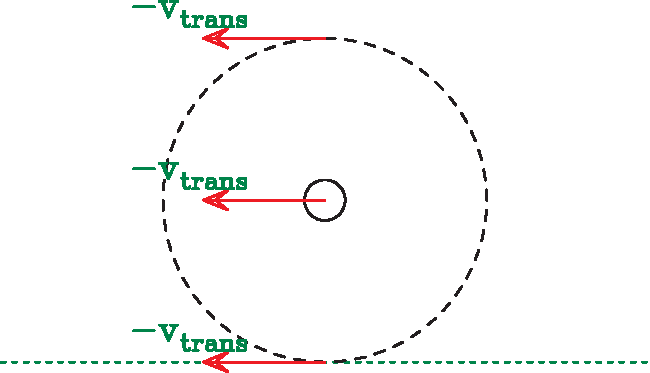
\includegraphics[width=0.32\textwidth]{roll-crop.pdf}
	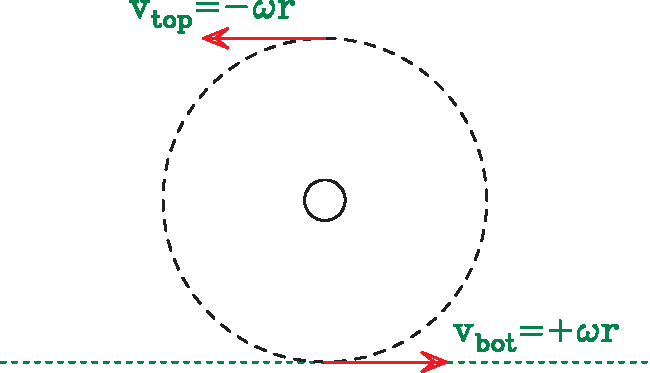
\includegraphics[width=0.32\textwidth]{roll2-crop.pdf}
	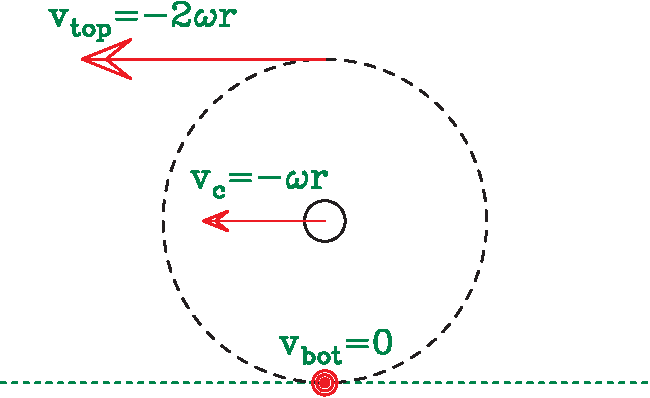
\includegraphics[width=0.32\textwidth]{roll3-crop.pdf}
	
	\Huge
	\begin{columns}
		\column{0.3\textwidth}
		Translation
		\column{0.3\textwidth}
		+ Rotation
		\column{0.3\textwidth}
		= Rolling
	\end{columns}
}


\frame{\frametitle{\textbf{The ``rolling constraint''}}
	
\Large
	
	If an object rolls forward on an edge of radius $r$,
	
	$$v = \omega r$$
	
	\BS\BS\pause
	
	Common algebra pattern:
	
	$$KE_{rot} = \frac{1}{2}{\color{Red}I} \omega^2$$
	
	$$KE_{rot} = \frac{1}{2}{\color{Red}\lambda m r^2} \omega^2$$
	
	$$KE_{rot} = \frac{1}{2}\lambda m {\color{Green}r^2 \omega^2}$$
	
		$$KE_{rot} = \frac{1}{2}\lambda m {\color{Green}v^2}$$
		
	}
	






\end{document}
